\section{网格布局}

CSS网格可以定义由行和列组成的二维布局,然后将元素放置到网格中。有些元素可能只占据网格的一个单元,另一些元素则可能占据多行或多列。网格的大小既可以精确定义,也可以根据自身内容自动计算。你既可以将元素精确地放置到网格某个位置,也可以让其在网格内自动定位,填充划分好的区域。

\subsection{网格布局基础}

网格布局和弹性布局类似,是两级 DOM 结构。设置为 \texttt{display: grid} 的元素成为一个网格容器。子元素成为网格元素。网格布局有如下概念:

\begin{figure}[H]
    \small
    \centering
    \begin{minipage}[t]{0.2\linewidth}
        \begin{tikzpicture}[scale = 1,ultra thick]
            \foreach \x in {0,0.75,1.5} {
                \foreach \y in {0,0.75} {
                    \draw[color = black!60, fill=black!10] (\x,\y) rectangle (\x+0.75,\y+0.75);
                }
            }
            \node at (1.125,-0.5) {网格线};
        \end{tikzpicture}
    \end{minipage}
    \begin{minipage}[t]{0.2\linewidth}
        \begin{tikzpicture}[scale = 1,ultra thick]
            \foreach \x in {0,0.75,1.5} {
                \draw[color = black!20, fill=black!10] (\x,0) rectangle (\x+0.75,0+0.75);
                \draw[color = black!20, fill=black!60] (\x,0.75) rectangle (\x+0.75,1.5);
            }
            \node at (1.125,-0.5) {网络轨道};
        \end{tikzpicture}
    \end{minipage}
    \begin{minipage}[t]{0.2\linewidth}
        \begin{tikzpicture}[scale = 1,ultra thick]
            \foreach \x in {0,0.75,1.5} {
                \foreach \y in {0,0.75} {
                    \draw[color = black!20, fill=black!10] (\x,\y) rectangle (\x+0.75,\y+0.75);
                }
            }
            \draw[color = black!20, fill=black!60] (0.75,0) rectangle (1.5,0.75);
            \node at (1.125,-0.5) {网络单元};
        \end{tikzpicture}
    \end{minipage}
    \begin{minipage}[t]{0.2\linewidth}
        \begin{tikzpicture}[scale = 1,ultra thick]
            \foreach \x in {0,0.75,1.5} {
                \foreach \y in {0,0.75} {
                    \draw[color = black!20, fill=black!10] (\x,\y) rectangle (\x+0.75,\y+0.75);
                }
            }
            \draw[color = black!20, fill=black!60] (0.75,0) rectangle (1.5,0.75);
            \draw[color = black!20, fill=black!60] (1.5,0) rectangle (2.25,0.75);
            \draw[color = black!20, fill=black!60] (0.75,0.75) rectangle (1.5,1.5);
            \draw[color = black!20, fill=black!60] (1.5,0.75) rectangle (2.25,1.5);
            \node at (1.125,-0.5) {网络区域};
        \end{tikzpicture}
    \end{minipage}
    \caption{网络的组成部分}
\end{figure}

网格容器有以下三个主要属性:

\begin{HTML}
.grid {
    display: grid;
    grid-template-column: 1fr 1fr 1fr;  /* 三列 */
    grid-template-rows: 1fr 1fr;        /* 两行 */
    grid-gap: 0.5em;                    /* 间隔 */
}
\end{HTML}

其中 \texttt{grid-template-column} 和 \texttt{grid-template-rows} 的数值和 \texttt{flex-grow} 类似,是用于计算权重的因子。

如果需要声明很多行/列,可以使用 \texttt{repeat()} 函数,接收两个参数,第一个为重复次数,第二个为重复的内容,例如 \texttt{repeat(3, 2fr 1fr)} 等价于 \texttt{2fr 1fr 2fr 1fr 2fr 1fr}。

网格元素有两个相关的属性:

\begin{HTML}
.element {
    grid-column: 1 / 3;  /* 1号竖网格线到3号竖网格线 */
    grid-row: span 1;    /* 占据第一条网格轨道 */
}
\end{HTML}

这两个属性有以上两种写法 \texttt{num/num} 表示占据哪两条网格线之间的网格,\texttt{span num} 则表示占据第几网格轨道。

具体的网格编号如下所示:

\begin{figure}[H]
    \small
    \centering
    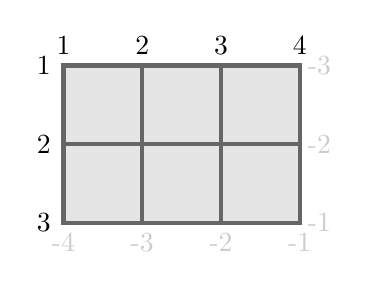
\begin{tikzpicture}[scale = 1,ultra thick]
        \foreach \x in {1,2,3} {
            \foreach \y in {1,2} {
                \draw[color = black!60, fill=black!10] (\x,\y) rectangle (\x+1,\y+1);
            }
        }
        \node at (1, 3.25) {1};
        \node at (2, 3.25) {2};
        \node at (3, 3.25) {3};
        \node at (4, 3.25) {4};
        \node at (0.75,1) {3};
        \node at (0.75,2) {2};
        \node at (0.75,3) {1};
        \begin{scope}[color = black!20]
            \node at (1, 0.75) {-4};
            \node at (2, 0.75) {-3};
            \node at (3, 0.75) {-2};
            \node at (4, 0.75) {-1};
            \node at (4.25,1) {-1};
            \node at (4.25,2) {-2};
            \node at (4.25,3) {-3};
        \end{scope}
    \end{tikzpicture}
    \caption{网格编号}
    \label{fig:网格编号}
\end{figure}

\subsubsection*{与 Flexbox 配合}

网格布局与弹性布局并不冲突,这两种布局方案几乎是一起开发出来的,不存在替代关系。Flexbox 本质上是一维布局,而 Grid 是二维布局。往往在网格中的部分网络区域使用 Flexbox 进行微操。

虽然 Flexbox 可以通过 \texttt{flex-wrap} 让元素换行进而达到伪二维的效果,但是这存在诸多弊端。一,\texttt{flex-wrap} 并不是为了二位布局而被设计出来的,而是为了兼容不同的设备与屏幕。二,\texttt{flex-wrap} 中换行的元素并不能达到很好的对齐效果,换行的元素往往是凌乱的。

网格布局时两级结构,每个网格元素都会扩展并填满整个网格区域,但是子元素不会,我们控制网格子元素时需要另行想办法控制高宽等属性,常饮用的方法就是使用 \texttt{Flexbox}。

\subsubsection*{替代语法}

布局网格元素还有另外两个替代语法:命名的网格线和命名的网格区域。

有时候记录所有网格线的编号实在太麻烦了,尤其是在处理很多网格轨道时。为了能简单点,可以给网格线命名,并在布局时使用网格线的名称而不是编号:

\begin{HTML}
grid-template-columns: [start] 2fr [center] 1fr [end];
\end{HTML}

这条声明定义了两列的网格,三条垂直的网格线分别叫作start、center和end。之后定义网格元素在网格中的位置时,可以不用编号而是用这些名称来声明:

\begin{HTML}
grid-column: start / center;
\end{HTML}

同时还可以给网格线提供多个名称:

\begin{HTML}
    grid-template-columns: [left-start] 2fr [left-end right-start] 1fr [right-end];
\end{HTML}

在这条声明里,2号网格线既叫作\texttt{left-end}也叫作\texttt{right-start},之后可以任选一个名称使用。这里还有一个彩蛋:将网格线命名为\texttt{left-start}和\texttt{left-end},就定义了一个叫作\texttt{left}的区域,这个区域覆盖两个网格线之间的区域。\texttt{-start}和\texttt{-end}后缀作为关键字,定义了两者之间的区域。如果给元素设置\texttt{grid-column: left},它就会跨越从\texttt{left-start}到\texttt{left-end}的区域。

此外还可以这样声明: \texttt{grid-template-columns: repeat(3, [col] 1fr 1fr)} 这样会出现三个 \texttt{col} 区域,使用 \texttt{grid-column: col 2 / span 2} (从第二个 \texttt{col} 开始跨越两个区域)可以定位到第二组网格列上。

命名网格区域不用计算或者命名网格线,直接用命名的网格区域将元素定位到网格中。实现这一方法需要借助网格容器的\texttt{grid-template-areas}属性和网格元素的\texttt{grid-area}属性。

\begin{HTML}
.container {   
    display: grid;   
    grid-template-areas: "title title"                       
                        "nav   nav"                        
                        "main  aside1"                        
                        "main  aside2";   
    grid-template-columns: 2fr 1fr;  
    grid-template-rows: repeat(4, auto); 
    grid-gap: 1.5em;   
    max-width: 1080px;   
    margin: 0 auto; 
} 
header {   
    grid-area: title;
} 
\end{HTML}

每个被命名的网格区域必须组成一个矩形。不能创造更复杂的形状。

还可以用句点(.)作为名称,这样便能空出一个网格单元。

\begin{HTML}
grid-template-areas: "top  top right"
                     "left . right"
                     "left bottom bottom";
\end{HTML}

网格布局共设计了三种语法:编号的网格线、命名的网格线、命名的网格区域。最后一个可能更受广大开发人员喜爱,尤其是明确知道每个网格元素的位置时,这种方式用起来更舒服。

\subsection{隐式网格}

当处理大量的网格元素时,挨个指定元素的位置未免太不方便。当元素是从数据库获取时,元素的个数可能是未知的。在这些情况下,以一种宽松的方式定义网格可能更合理,剩下的交给布局算法来放置网格元素。

这时需要用到隐式网格(implicit  grid)。使用\texttt{grid-template-*}属性定义网格轨道时,创建的是显式网格(explicit  grid),但是有些网格元素仍然可以放在显式轨道外面,此时会自动创建隐式轨道以扩展网格,从而包含这些元素。

如果网格元素放在声明的网格轨道之外,就会创建隐式轨道,直到包含该元素。

隐式网格轨道默认大小为\texttt{auto},也就是它们会扩展到能容纳网格元素内容。可以给网格容器设置\texttt{grid-auto-columns}和\texttt{grid-auto-rows},为隐式网格轨道指定一个大小(比如,\texttt{grid-auto-columns: 1fr})。

使用隐式网络时,由于不确定元素数量,可以给 \texttt{grid-template-columns} 使用 \texttt{auto-fill} 值,代表会根据屏幕宽度自动设置列数量,配合 \texttt{minmax()} 函数可以有效地适配各种屏幕分辨率。如果网格元素不够填满所有网格轨道,\texttt{auto-fill}就会导致一些空的网格轨道。如果不希望出现空的网格轨道,可以使用\texttt{auto-fit}关键字代替\texttt{auto-fill}。它会让非空的网格轨道扩展,填满可用空间。

\subsubsection*{添加变化}

熟悉 Win10 磁铁的读者肯定知道磁铁的大小可以改变,网格布局也可以改变为 2x1, 2x2 大小。网格布局提供了一个属性\texttt{grid-auto-flow},它可以控制布局算法的行为。它的初始值是\texttt{row},如果值为\texttt{column},它就会将元素优先放在网格列中,只有当一列填满了,才会移动到下一行。

但是这样存在一定的问题,无论按行还是按列,有时候大网格区域后紧跟的小网格区域会造成很多空网格单元,只需要为 \texttt{grid-auto-flow} 添加 \texttt{dense} 值即可,小元素就会“回填”大元素造成的空白区域。代价是会改变元素的排列顺序。

\subsubsection*{对齐}

最后讲一下对齐,针对主轴和副轴有两种对齐属性,分别以 \texttt{justify} 和 \texttt{align} 开头,对象有所不同,如下表所示:

\begin{table}[H]
    \centering
    \caption{网格对其属性}
    \label{table:网格对其属性}
    \setlength{\tabcolsep}{4mm}
    \begin{tabular}{c|ccc}
        \toprule
        \textbf{属性} & \textbf{作用于} & \textbf{对齐} \\
        \midrule
        \texttt{justify-items, align-items} & 网络容器 & 网格区域内的所有元素 \\
        \texttt{justify-self, align-self} & 网络元素 & 网格区域内的单个元素 \\
        \texttt{justify-content, align-content} & 网络容器 & 网格区域内的网络轨道 \\
        \bottomrule
    \end{tabular}
\end{table}

它们属性值和 Flexbox 类似。

\newpage